% Niveau :      PCSI
% Discipline :  Méca

\begin{exercise}{Flambage}{3}{Sup}
{Mécanique,Ressort}{lelay}

\textsl{Le but de cet exercice est de modéliser de manière simple l'instabilité de flambage. C'est ce qui se produit par exemple lorsqu'on compresse une règle en plastique à ses extrémités.}

On considère deux murs verticaux situés en $x = \pm a$. Une masse $m$ est reliée à chacun des murs par un ressort de raideur $k$ et de longueur à vide $\ell_0$ dont les points d'attache sont situés face à face.
\begin{questions}
    \questioncours Définition d'un point d'équilibre stable, instable.
    \question Montrez qualitativement que si la masse est initialement centrée en $x=0$, elle y restera tout le temps. On considérera cette condition comme vérifiée par la suite.
    \uplevel{On considère dans un premier temps que la masse n'est pas soumise à son poids ($g = 0$).}
    \question On considère le cas $a > \ell_0$. Appliquer le PFD à la masse.
    \begin{parts}
        \part Combien y a-t-il de points d'équilibre ?
        \part Donner l'équation horaire du mouvement de la masse en considérant qu'elle commence son mouvement à $t=0$ proche d'un point d'équilibre et sans vitesse initiale.
    \end{parts}
    \question On considère le cas $a < \ell_0$. Écrire l'énergie potentielle de la masse.
    \begin{parts}
        \part Combien y a-t-il de points d'équilibre ?
        \part Donner l'équation horaire du mouvement de la masse en considérant qu'elle commence son mouvement à $t=0$ proche d'un point d'équilibre et sans vitesse initiale.
    \end{parts}
    \question Représenter sur un graphe les points d'équilibres (sous forme adimensionnée $u=z_{eq}/\ell_0$) en fonction de $r = a/\ell_0$.
    \question On s'intéresse maintenant à la stabilité de ces points d'équilibre. Rappeler comment déterminer la stabilité d'un point d'équilibre. 
    \begin{parts}
        \part On considère le cas $a > \ell_0$. Combien de points d'équilibre y a-t-il ? Quelle est leur stabilité ?
        \part On considère le cas $a < \ell_0$. Combien de points d'équilibre y a-t-il ? Quelle est leur stabilité ?
        \part Redessiner le graphe $u = f(r)$ en prenant compte de la stabilité des points. Pourquoi appelle-t-on cette bifurcation \textit{fourche} super critique ?
    \end{parts}
    \uplevel{On considère maintenant que la bille est soumise à son poids ($g \neq 0$).}
    \question À votre avis, qu'est-ce que cela va changer au problème ? 
    \question On considère une bille de faible poids. Comment quantifier physique cette affirmation ?
    \begin{parts}
        \part On suppose maintenant que le rail est incliné d'un angle $\alpha$ par rapport à l'horizontale. Montrer que l'équation que vérifient les points fixes donne sous forme adimensionnée :
        \begin{align*}
            1+\frac{h}u = \frac{r}{\sqrt{1+u^2}}
        \end{align*}
        où $h$ est une constante à déterminer.
        \part En supposant $u \ll 1$, montrer que cette équation se réduit à $\frac{u^3}{2r^3}+h = \frac{1-r}{r}u$. En prenant $h \ll 1$, dessiner les graphes des fonctions $u \mapsto u^3+h$ et $u\mapsto (r-1)u$ pour $r > 1$ et $r<1$. 
        \part En déduire l'allure du graphe $u = f(r)$. Qu'est ce qui a changé par rapport à la situation précédente ? 
        \part Pour un $r>1$ donné, représenter l'allure de $u = f(h)$. Pouvez-vous expliquer pourquoi l'ajout de $g$ est \textit{catastrophique} ?
    \end{parts}
    \question Que se passe-t-il  si $g$ est grand ?
\end{questions}

% \begin{figure}{H}
%     \centering
%     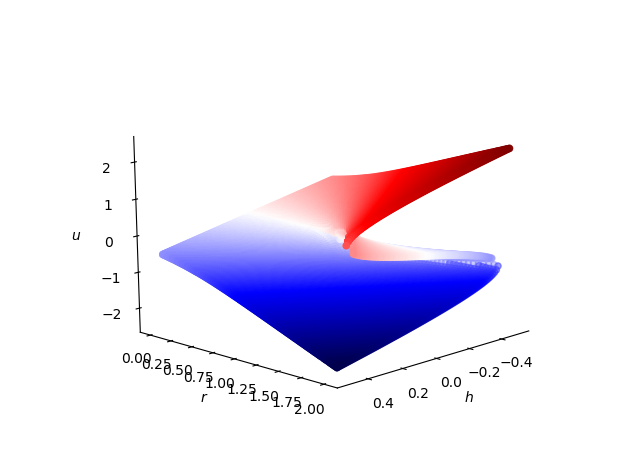
\includegraphics[height=15em]{meca/mecapoint/fourchevraie.png}
%     \caption{Vision pas d'artiste d'une bifurcation fourche supercritique.}
% \end{figure}

% \begin{figure}{H}
%     \centering
%     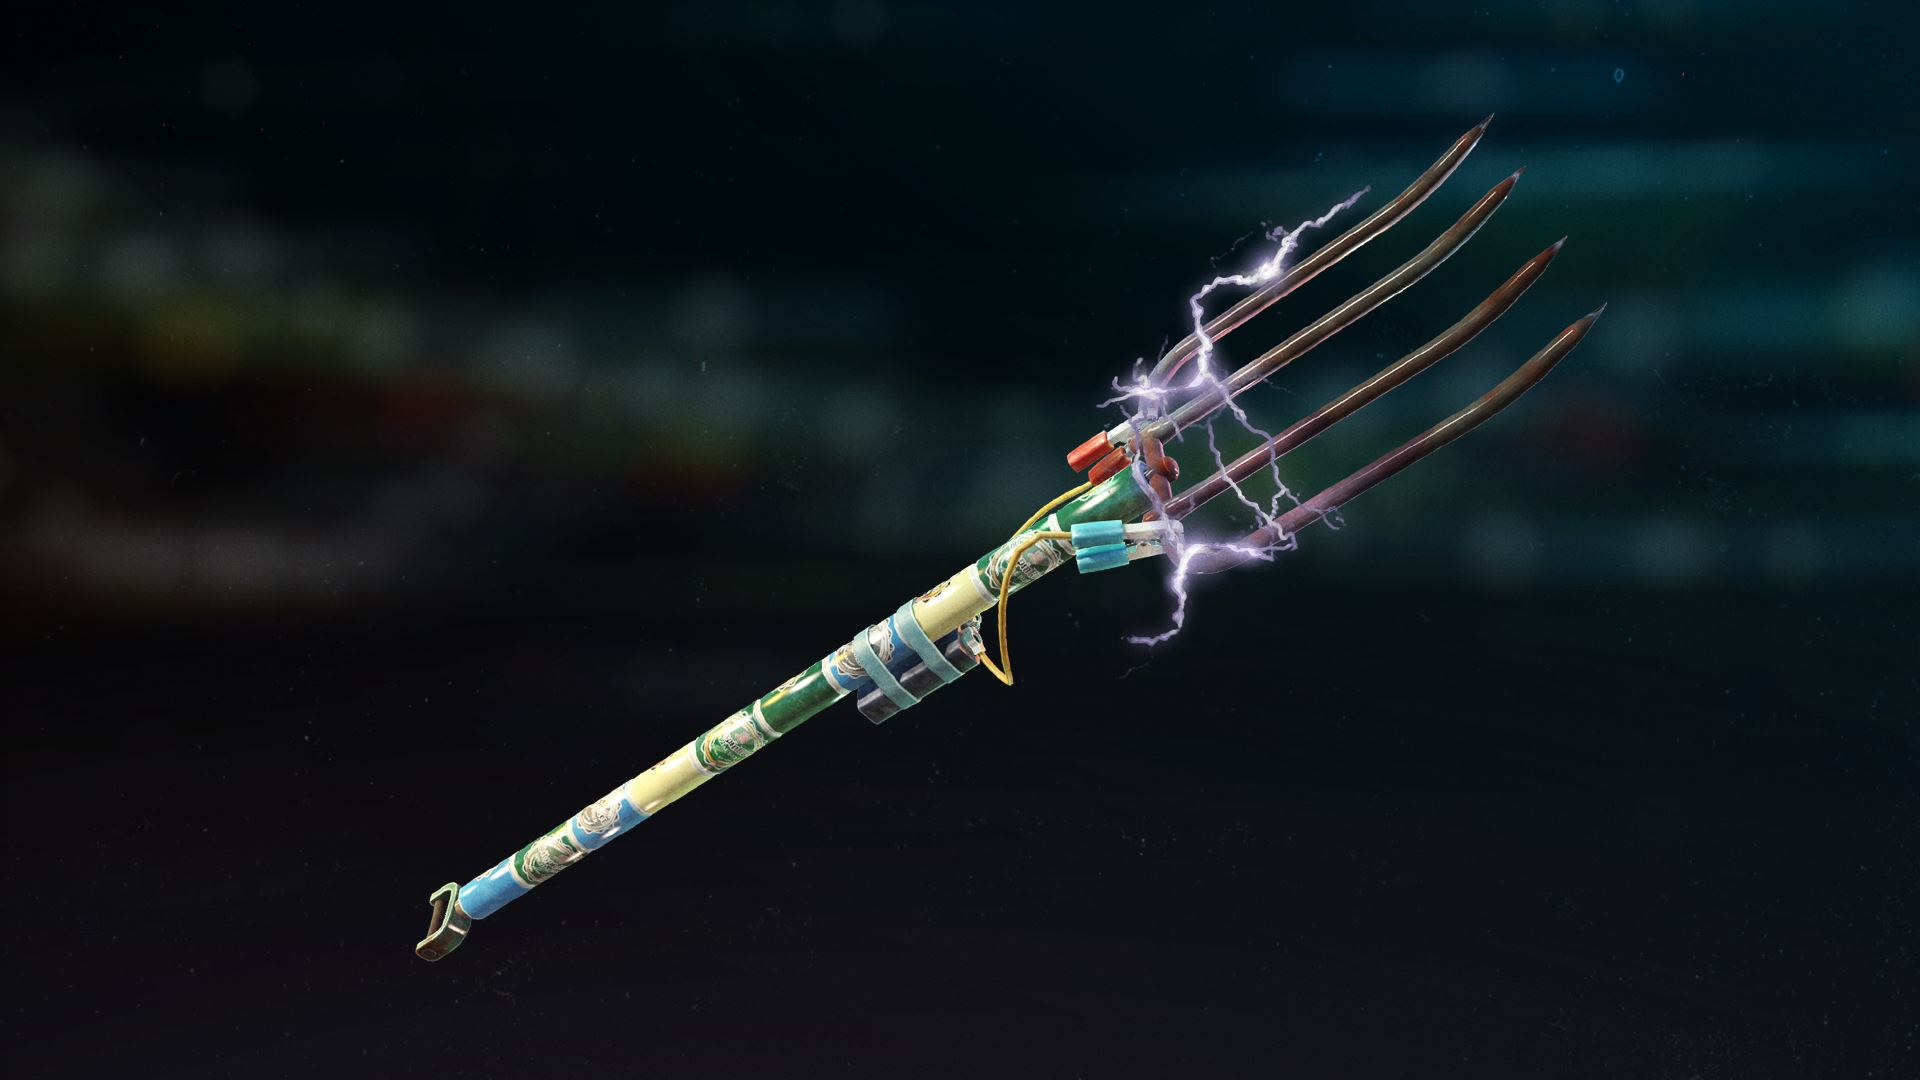
\includegraphics[height=15em]{meca/mecapoint/fourchesupercritique.jpg}%non ! siii ! %gros vilain !
%     \caption{Vision d'artiste d'une fourche supercritique.}
% \end{figure}

\end{exercise}